\begin{frame}
  \tableofcontents[currentsection]
\end{frame}

\begin{frame}{Chaîne d'acquisition}
  \framesubtitle{Amplification et polarisation du signal audio}
  \begin{columns}[c]
  \column{.25\textwidth}
  \vspace{4.5cm}
  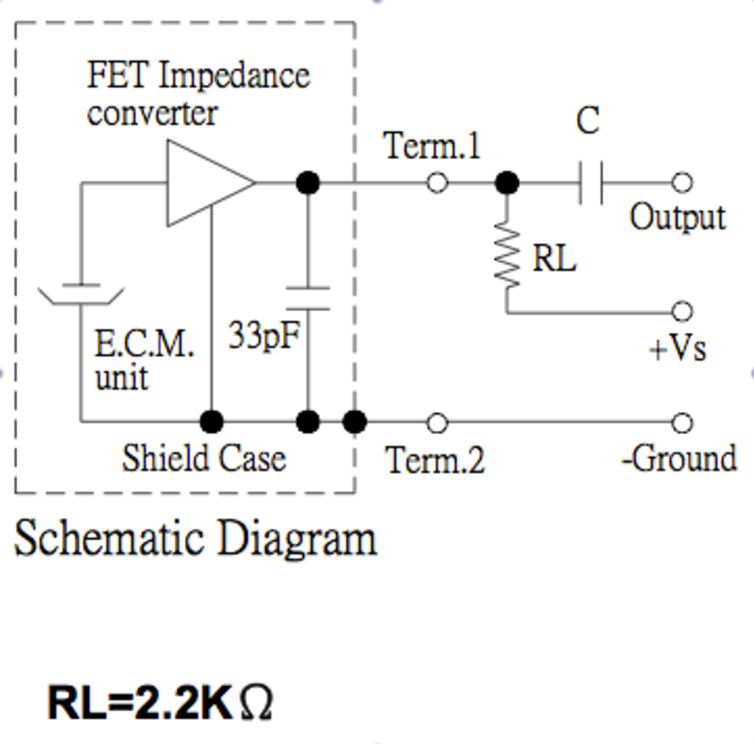
\includegraphics[width = \textwidth]{polarisation_micro.pdf}
  \column{.9\textwidth}
  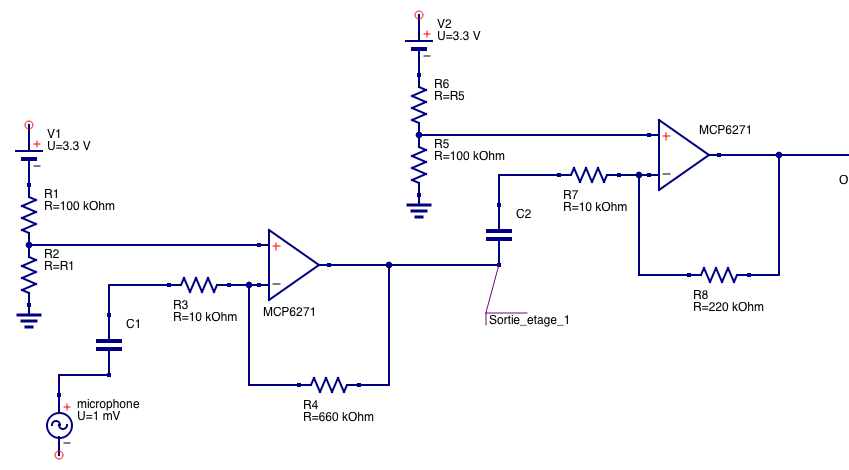
\includegraphics[width = \textwidth]{etage_amplificateur.png}
  \end{columns}
\end{frame}

\begin{frame}{Chaîne d'acquisition}
  \framesubtitle{Filtre de garde}
  \begin{columns}[c]
  \column{.7\textwidth}
  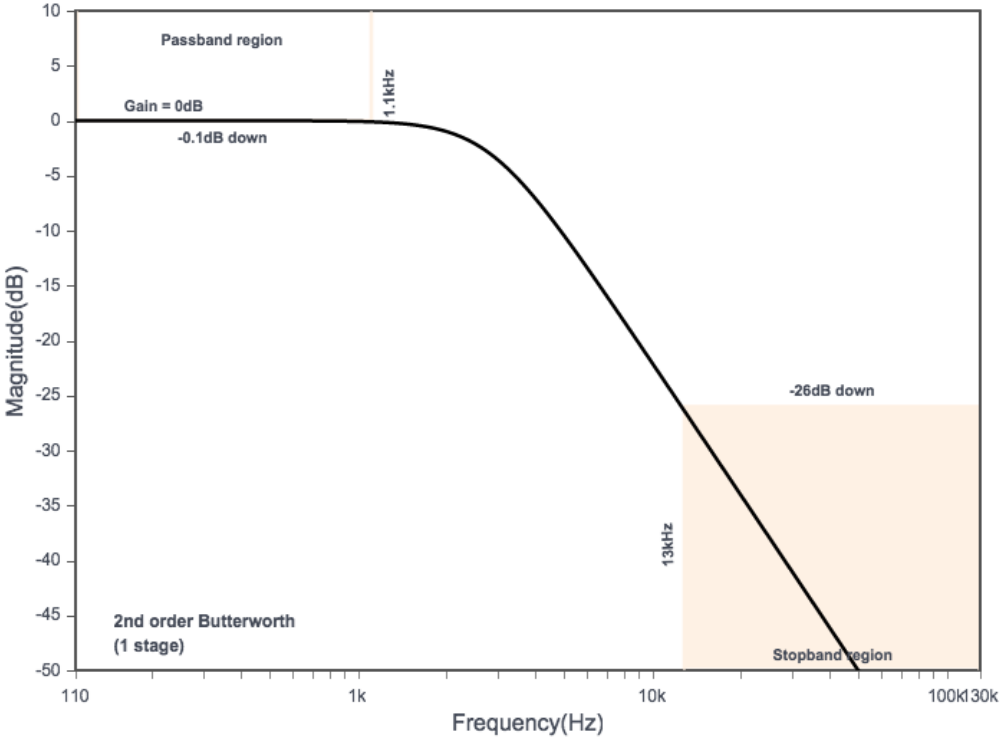
\includegraphics[width = \textwidth]{repFreqFiltreAnalog.png}
  \column{.45\textwidth}
  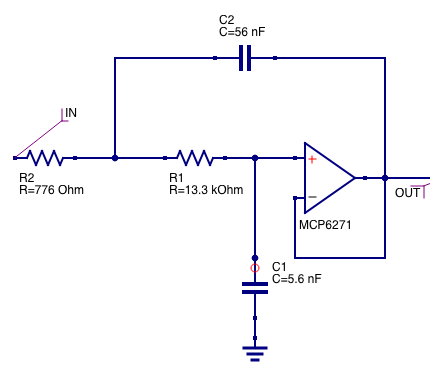
\includegraphics[width = \textwidth]{filtre_analogique.png}
  \end{columns}
\end{frame}

\begin{frame}{Traitement numérique du signal}
  \framesubtitle{Filtres passe-bande}
  \begin{center}
  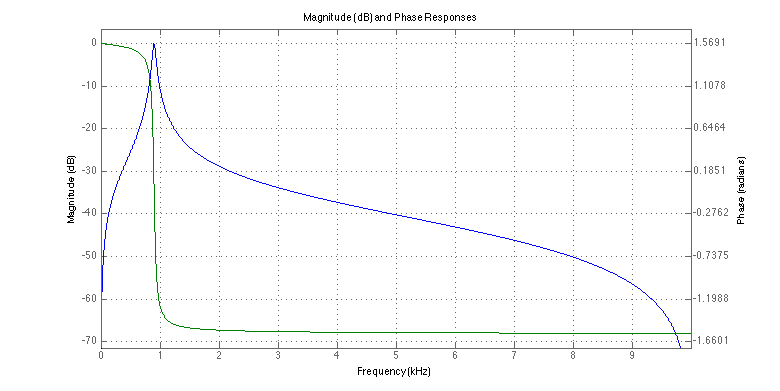
\includegraphics[width = 1\textwidth]{filtre_1section.png}\\
  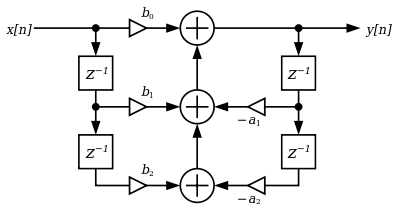
\includegraphics[width = .35\textwidth]{filtre_bloc.png}
  \end{center}
\end{frame}

\begin{frame}{Traitement numérique du signal}
  \framesubtitle{Détection de crête -- intégration avec \ilcode{fskDetector}}
  \begin{itemize}
    \item Crête détectée si le maximum sur les derniers échantillons correspondant à une période de signal est supérieur à un niveau minimal
    \item Routine d'échantillonnage:
    \begin{itemize}
      \item Filtrage $\rightarrow$ deux échantillons filtrés
      \item Détection de crête $\rightarrow$ deux booléens
      \item Détection de trame FSK $\rightarrow$ trame reconstituée ou rien
    \end{itemize}
    {\large $\Rightarrow$ Temps d'exécution $<1/\mathsf{f_s}$!?}
    \item Si une trame est reconstituée, elle est ensuite passée au bloc UART
  \end{itemize}
\end{frame}



